\documentclass[10pt,a4paper,landscape]{article}
\usepackage[T1]{fontenc}
\usepackage[margin=1.6cm]{geometry}
\usepackage{underscore}
\usepackage{booktabs,array,graphicx}
\usepackage{tikz}
\usetikzlibrary{arrows.meta,positioning,calc}
\setlength{\parindent}{0pt}
\setlength{\parskip}{4pt}
\pagestyle{empty}

\tikzset{
  >={Stealth[length=3mm,width=2.4mm]},
  box/.style={draw,rounded corners=2pt,align=center,fill=blue!6,font=\small,inner sep=4pt},
  mem/.style={box,fill=green!10},
  reg/.style={draw,align=center,fill=green!15,font=\small,inner sep=4pt},
  mux/.style={draw,align=center,fill=yellow!20,font=\scriptsize,inner sep=3pt},
  op/.style={draw,circle,minimum size=0.9cm,fill=orange!15,font=\small},
  data/.style={->,line width=0.9pt},
  ctrl/.style={->,dashed,line width=0.7pt},
  lab/.style={font=\scriptsize,fill=white,inner sep=1pt,align=center},
  lbs/.style={font=\tiny,fill=white,inner sep=1pt,align=center}
}

\begin{document}

%==========================================================================
{\Large\bfseries 1. High-level schematic}\quad{\small Solid arrows carry data, dashed arrows carry control from the FSM.}

\medskip
\begin{center}
\resizebox{\textwidth}{!}{%
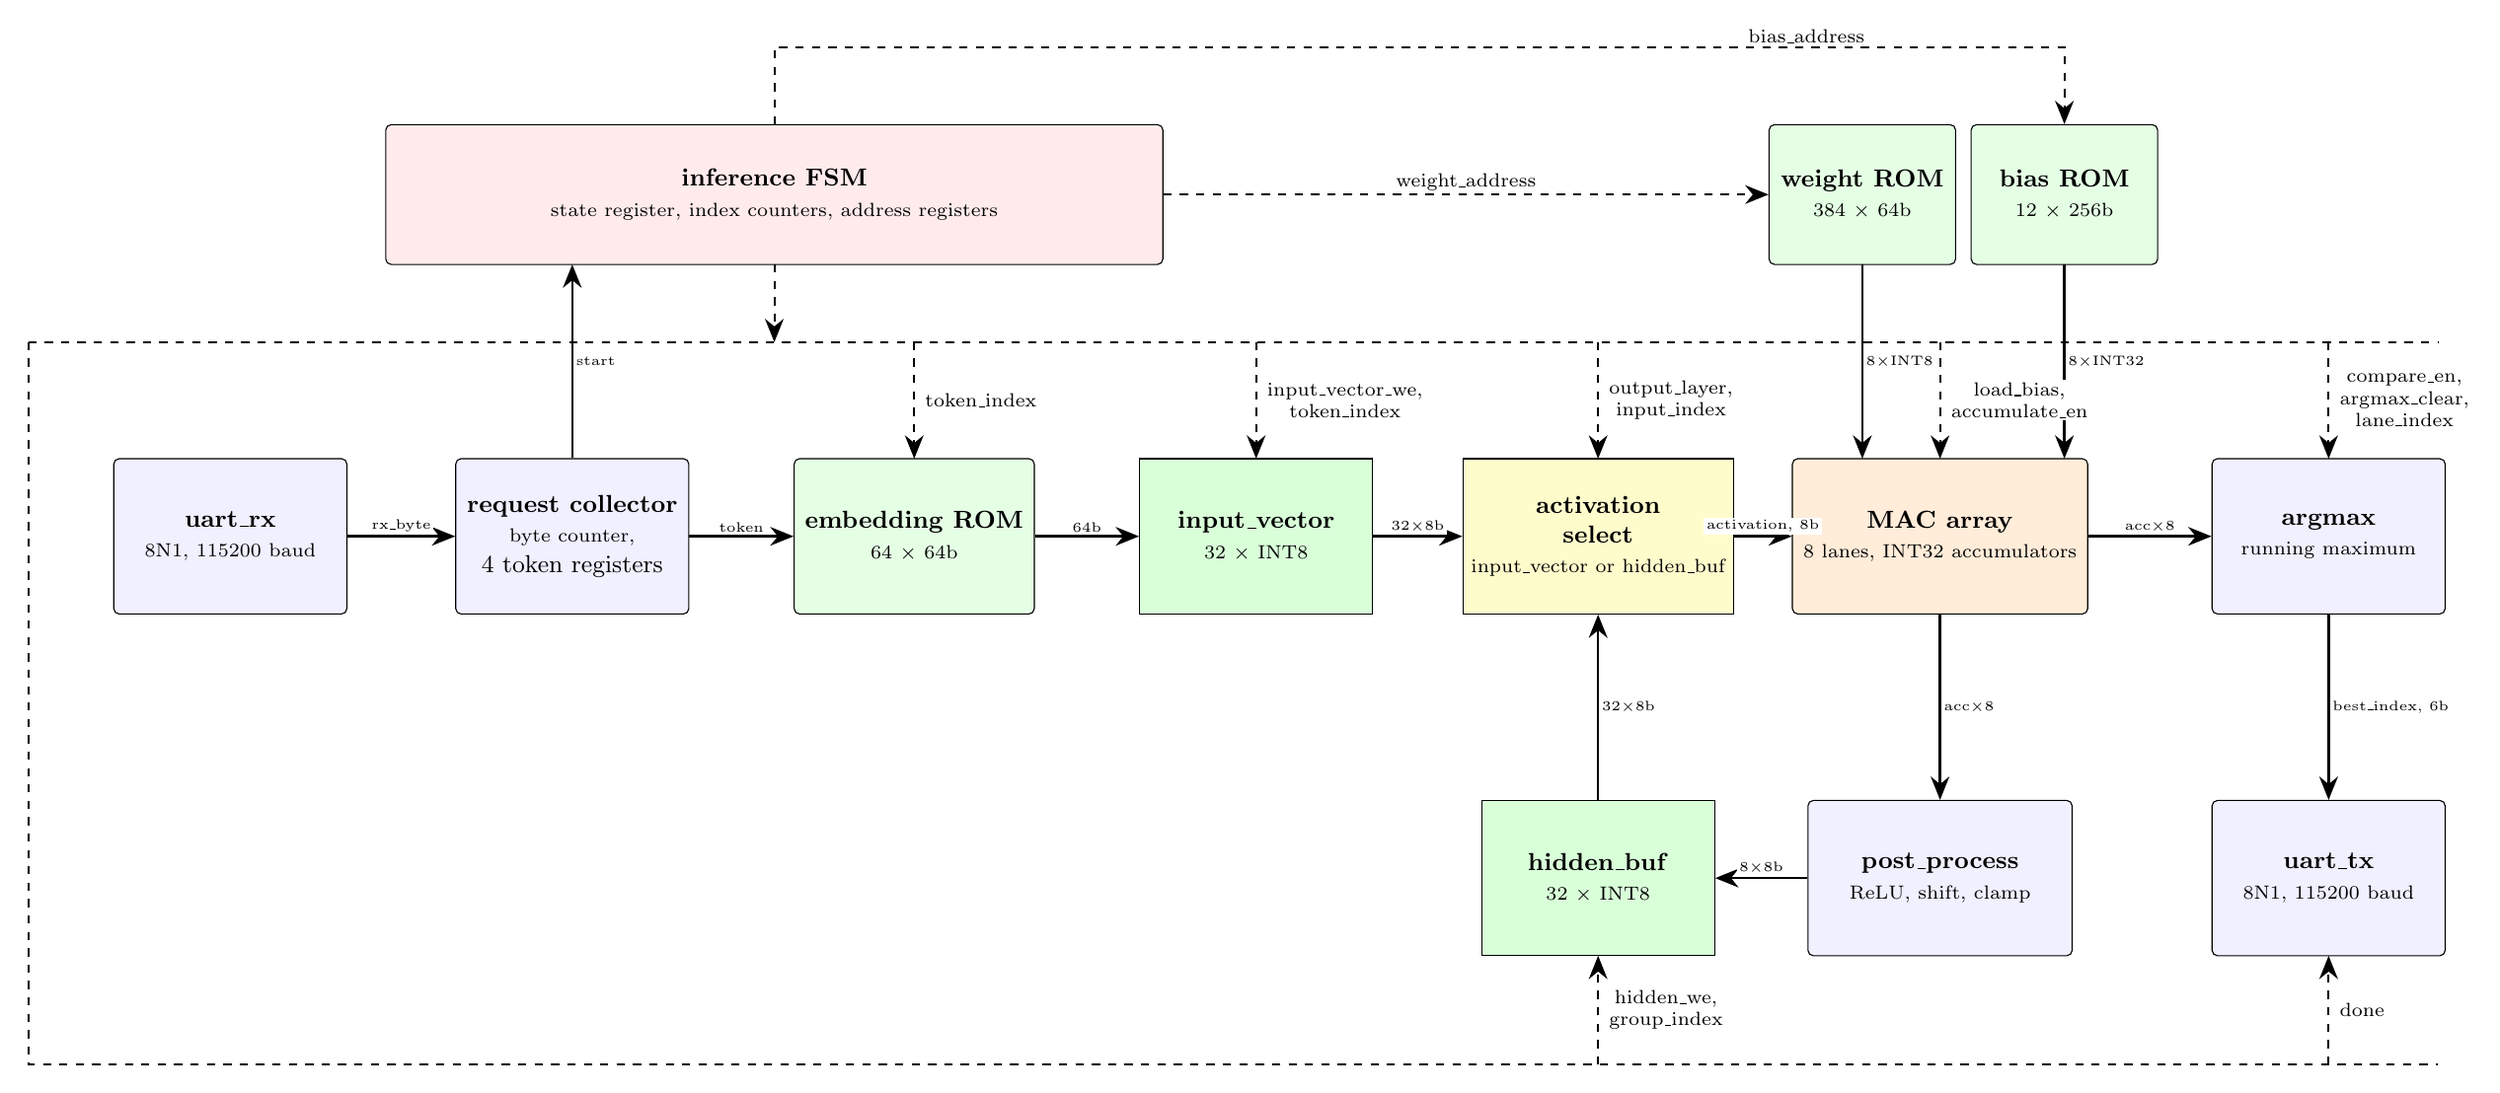
\begin{tikzpicture}
\node[box,minimum width=3.0cm,minimum height=2.0cm] (rx)  at (0,0)    {\textbf{uart_rx}\\{\scriptsize 8N1, 115200 baud}};
\node[box,minimum width=3.0cm,minimum height=2.0cm] (col) at (4.4,0)  {\textbf{request collector}\\\scriptsize byte counter,\\4 token registers};
\node[mem,minimum width=3.0cm,minimum height=2.0cm] (er)  at (8.8,0)  {\textbf{embedding ROM}\\{\scriptsize 64 $\times$ 64b}};
\node[reg,minimum width=3.0cm,minimum height=2.0cm] (xb)  at (13.2,0) {\textbf{input_vector}\\{\scriptsize 32 $\times$ INT8}};
\node[mux,minimum width=3.0cm,minimum height=2.0cm,font=\small] (as) at (17.6,0) {\textbf{activation}\\\textbf{select}\\{\scriptsize input_vector or hidden_buf}};
\node[box,minimum width=3.8cm,minimum height=2.0cm,fill=orange!15] (mac) at (22.0,0) {\textbf{MAC array}\\{\scriptsize 8 lanes, INT32 accumulators}};
\node[box,minimum width=3.0cm,minimum height=2.0cm] (am)  at (27.0,0)  {\textbf{argmax}\\{\scriptsize running maximum}};

\node[reg,minimum width=3.0cm,minimum height=2.0cm] (hb) at (17.6,-4.4) {\textbf{hidden_buf}\\{\scriptsize 32 $\times$ INT8}};
\node[box,minimum width=3.4cm,minimum height=2.0cm] (pp) at (22.0,-4.4) {\textbf{post_process}\\{\scriptsize ReLU, shift, clamp}};
\node[box,minimum width=3.0cm,minimum height=2.0cm] (tx) at (27.0,-4.4) {\textbf{uart_tx}\\{\scriptsize 8N1, 115200 baud}};

\node[mem,minimum width=2.4cm,minimum height=1.8cm] (wr) at (21.0,4.4) {\textbf{weight ROM}\\{\scriptsize 384 $\times$ 64b}};
\node[mem,minimum width=2.4cm,minimum height=1.8cm] (br) at (23.6,4.4) {\textbf{bias ROM}\\{\scriptsize 12 $\times$ 256b}};
\node[box,minimum width=10cm,minimum height=1.8cm,fill=red!8] (fsm) at (7.0,4.4) {\textbf{inference FSM}\\{\scriptsize state register, index counters, address registers}};

\draw[data] (rx) -- node[above,lbs]{rx_byte} (col);
\draw[data] (col) -- node[above,lbs]{token} (er);
\draw[data] (er) -- node[above,lbs]{64b} (xb);
\draw[data] (xb) -- node[above,lbs]{32$\times$8b} (as);
\draw[data] (as) -- node[above,lbs]{activation, 8b} (mac);
\draw[data] (mac) -- node[above,lbs]{acc$\times$8} (am);
\draw[data] (mac) -- node[right,lbs]{acc$\times$8} (pp);
\draw[data] (pp) -- node[above,lbs]{8$\times$8b} (hb);
\draw[data] (hb) -- node[right,lbs]{32$\times$8b} (as);
\draw[data] (am) -- node[right,lbs]{best_index, 6b} (tx);
\draw[data] (21.0,3.5) -- node[right,lbs]{8$\times$INT8} (21.0,1.0);
\draw[data] (23.6,3.5) -- node[right,lbs]{8$\times$INT32} (23.6,1.0);
\draw[data] (col.north) -- node[right,lbs]{start} (4.4,3.5);

\draw[ctrl,-] (-2.6,2.5) -- (28.4,2.5);
\draw[ctrl,-] (-2.6,2.5) -- (-2.6,-6.8) -- (28.4,-6.8);
\draw[ctrl] (7.0,3.5) -- (7.0,2.5);
\foreach \x/\t in {8.8/{token_index},13.2/{input_vector_we,\\token_index},17.6/{output_layer,\\input_index},22.0/{load_bias,\\accumulate_en},27.0/{compare_en,\\argmax_clear,\\lane_index}}{
  \draw[ctrl] (\x,2.5) -- (\x,1.0);
  \node[lab,anchor=west] at (\x+0.1,1.75) {\t};
}
\foreach \x/\t in {17.6/{hidden_we,\\group_index},27.0/{done}}{
  \draw[ctrl] (\x,-6.8) -- (\x,-5.4);
  \node[lab,anchor=west] at (\x+0.1,-6.1) {\t};
}
\draw[ctrl] (fsm.east) -- node[above,lab]{weight_address} (wr.west);
\draw[ctrl] (fsm.north) -- (7.0,6.3) -- node[pos=0.8,above,lab]{bias_address} (23.6,6.3) -- (br.north);
\end{tikzpicture}}
\end{center}

{\small The collector assembles four UART bytes into four 6-bit token registers and raises \texttt{start}. The FSM then walks the datapath: embedding lookup into \texttt{input_vector}, the hidden layer into \texttt{hidden_buf}, the output layer into the argmax, and finally \texttt{done} triggers \texttt{uart_tx}. The hidden and output layers use the same activation select, ROMs, and MAC array; only \texttt{output_layer} changes which buffer feeds the activation select.}

\clearpage
%==========================================================================
{\Large\bfseries 2. Low level: input side (embedding, buffers, activation select, ROMs)}

\medskip
\begin{center}
\resizebox{\textwidth}{!}{%
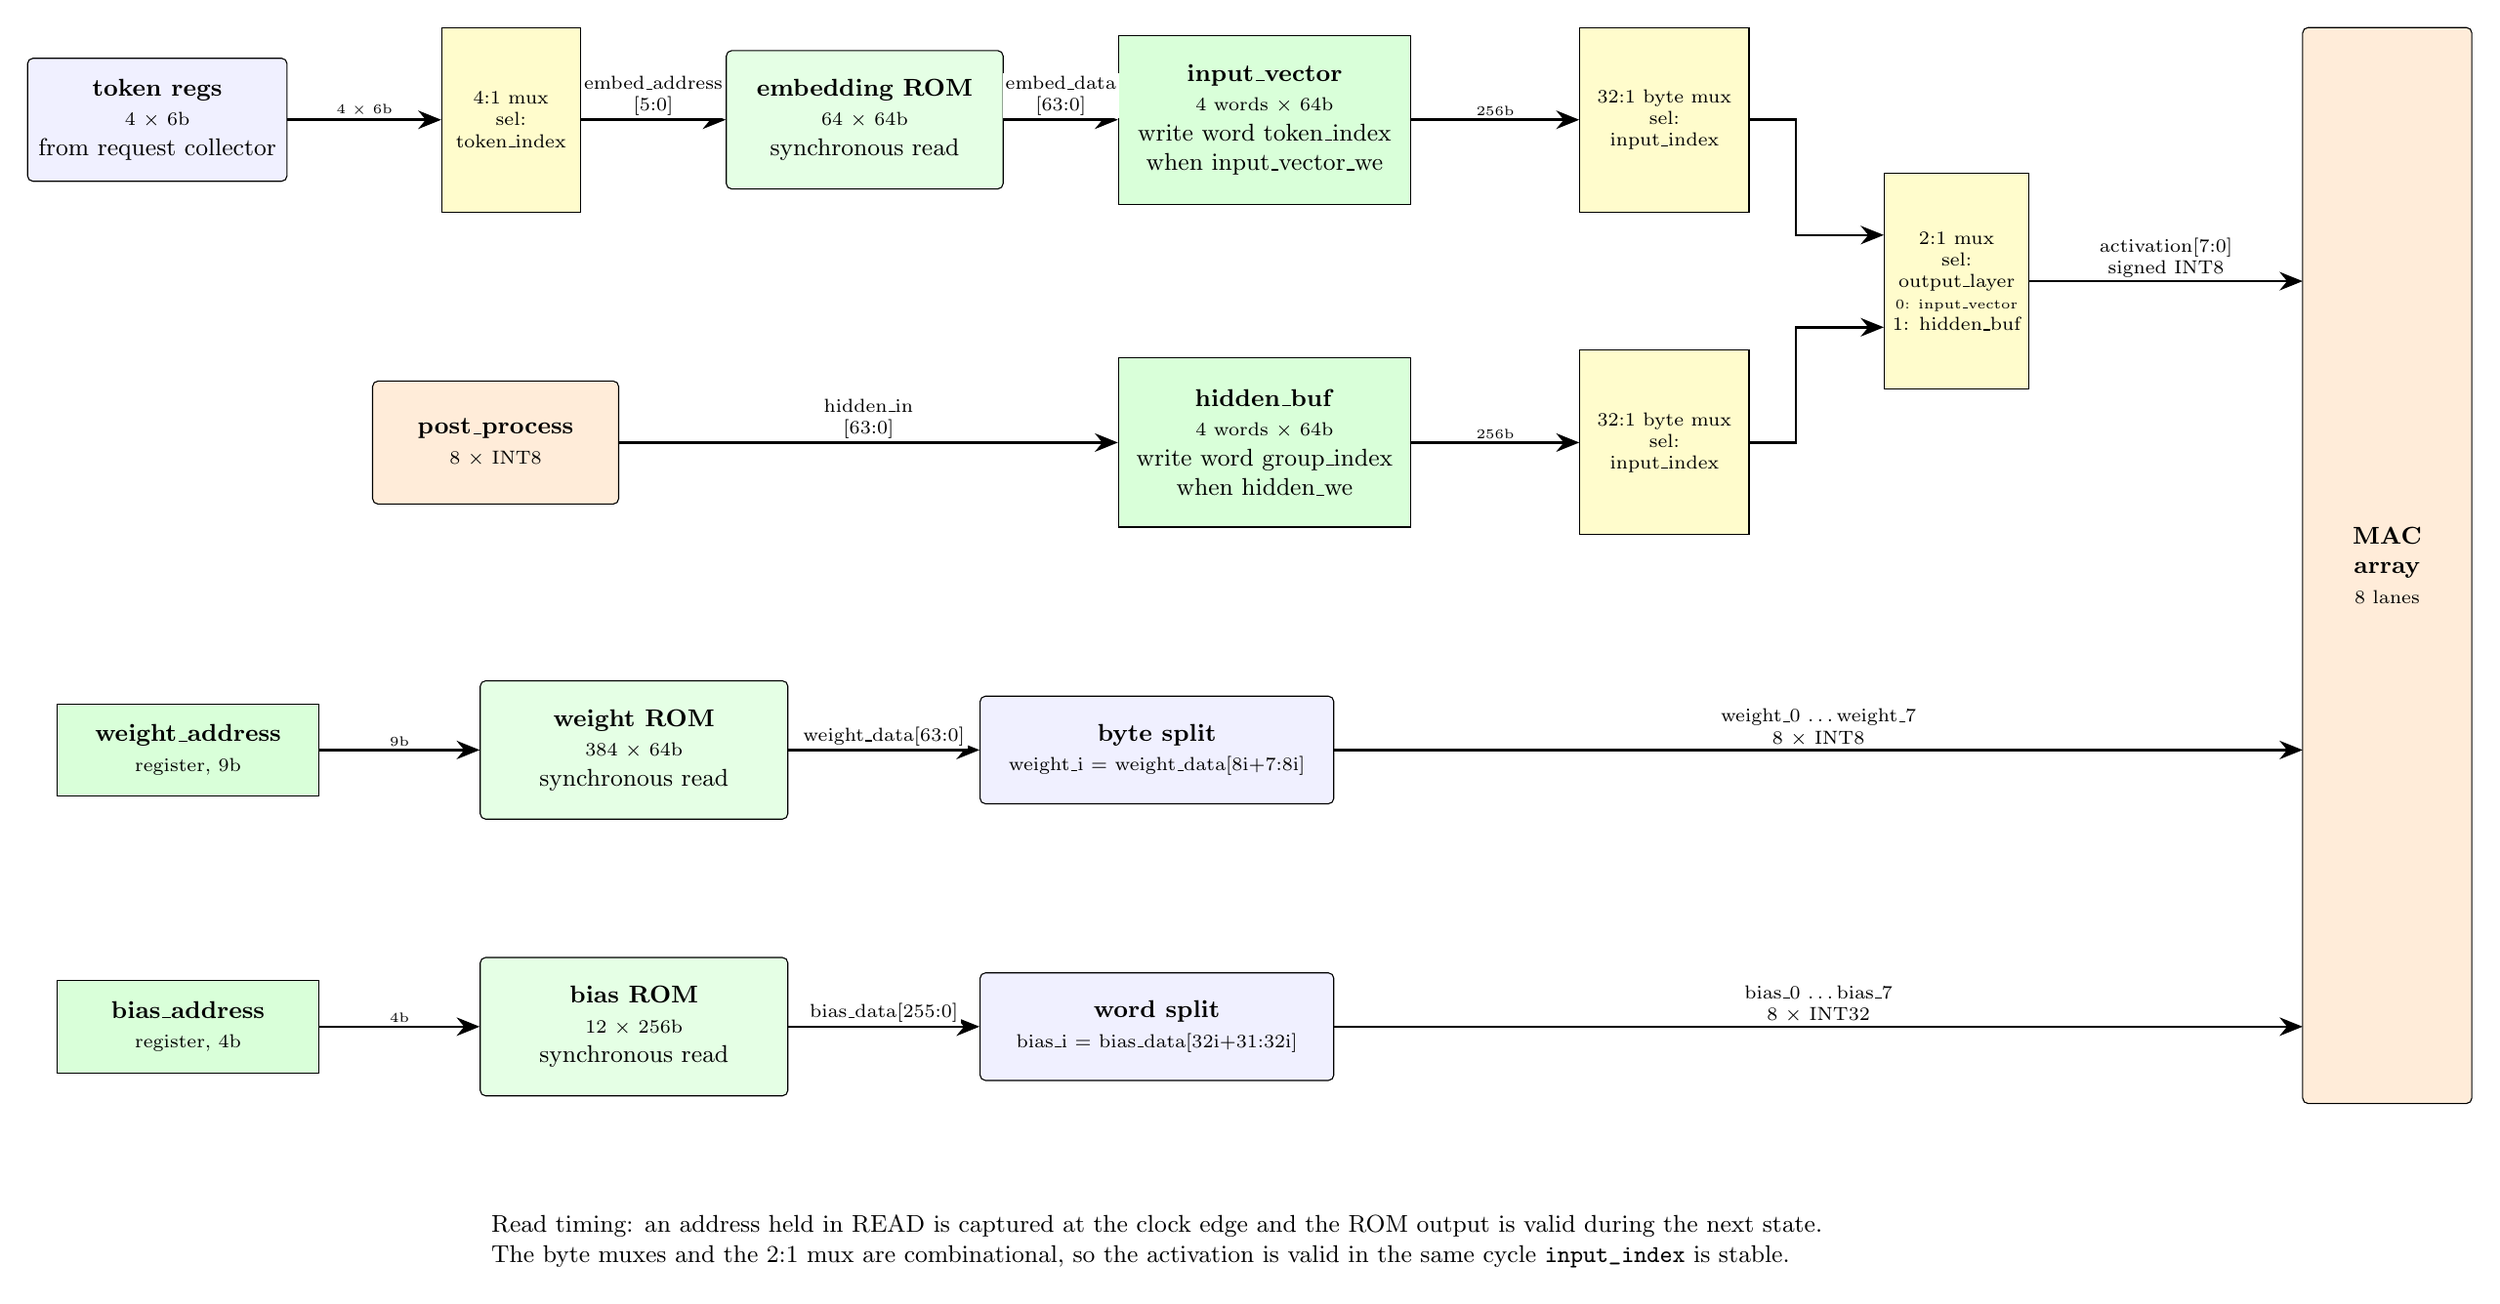
\begin{tikzpicture}
\node[box,minimum width=3.2cm,minimum height=1.6cm] (tok) at (0,6.2) {\textbf{token regs}\\\scriptsize 4 $\times$ 6b\\from request collector};
\node[mux,minimum width=1.8cm,minimum height=2.4cm] (mt) at (4.6,6.2) {4:1 mux\\sel:\\token_index};
\node[mem,minimum width=3.6cm,minimum height=1.8cm] (er) at (9.2,6.2) {\textbf{embedding ROM}\\\scriptsize 64 $\times$ 64b\\synchronous read};
\node[reg,minimum width=3.8cm,minimum height=2.2cm] (xb) at (14.4,6.2) {\textbf{input_vector}\\\scriptsize 4 words $\times$ 64b\\write word token_index\\when input_vector_we};
\node[box,minimum width=3.2cm,minimum height=1.6cm,fill=orange!15] (pp) at (4.4,2.0) {\textbf{post_process}\\{\scriptsize 8 $\times$ INT8}};
\node[reg,minimum width=3.8cm,minimum height=2.2cm] (hb) at (14.4,2.0) {\textbf{hidden_buf}\\\scriptsize 4 words $\times$ 64b\\write word group_index\\when hidden_we};
\node[mux,minimum width=2.2cm,minimum height=2.4cm] (m0) at (19.6,6.2) {32:1 byte mux\\sel:\\input_index};
\node[mux,minimum width=2.2cm,minimum height=2.4cm] (m1) at (19.6,2.0) {32:1 byte mux\\sel:\\input_index};
\node[mux,minimum width=1.8cm,minimum height=2.8cm] (ml) at (23.4,4.1) {2:1 mux\\sel:\\output_layer\\\tiny 0: input_vector\\1: hidden_buf};

\draw[data] (tok) -- node[above,lbs]{4 $\times$ 6b} (mt);
\draw[data] (mt) -- node[above,lab]{embed_address\\{[5:0]}} (er);
\draw[data] (er) -- node[above,lab]{embed_data\\{[63:0]}} (xb);
\draw[data] (xb) -- node[above,lbs]{256b} (m0);
\draw[data] (hb) -- node[above,lbs]{256b} (m1);
\draw[data] (pp) -- node[above,lab]{hidden_in\\{[63:0]}} (hb);
\draw[data] (m0.east) -- ++(0.6,0) |- ([yshift=0.6cm]ml.west);
\draw[data] (m1.east) -- ++(0.6,0) |- ([yshift=-0.6cm]ml.west);
\draw[data] (ml.east) -- node[above,lab]{activation[7:0]\\signed INT8} (27.9,4.1);

\node[reg,minimum width=3.4cm,minimum height=1.2cm] (wa) at (0.4,-2.0) {\textbf{weight_address}\\{\scriptsize register, 9b}};
\node[mem,minimum width=4.0cm,minimum height=1.8cm] (wrom) at (6.2,-2.0) {\textbf{weight ROM}\\\scriptsize 384 $\times$ 64b\\synchronous read};
\node[box,minimum width=4.6cm,minimum height=1.4cm] (wsp) at (13.0,-2.0) {\textbf{byte split}\\{\scriptsize weight_i = weight_data[8i+7:8i]}};
\draw[data] (wa) -- node[above,lbs]{9b} (wrom);
\draw[data] (wrom) -- node[above,lab]{weight_data[63:0]} (wsp);
\draw[data] (wsp.east) -- node[above,lab]{weight_0 \dots weight_7\\8 $\times$ INT8} (27.9,-2.0);

\node[reg,minimum width=3.4cm,minimum height=1.2cm] (ba) at (0.4,-5.6) {\textbf{bias_address}\\{\scriptsize register, 4b}};
\node[mem,minimum width=4.0cm,minimum height=1.8cm] (brom) at (6.2,-5.6) {\textbf{bias ROM}\\\scriptsize 12 $\times$ 256b\\synchronous read};
\node[box,minimum width=4.6cm,minimum height=1.4cm] (bsp) at (13.0,-5.6) {\textbf{word split}\\{\scriptsize bias_i = bias_data[32i+31:32i]}};
\draw[data] (ba) -- node[above,lbs]{4b} (brom);
\draw[data] (brom) -- node[above,lab]{bias_data[255:0]} (bsp);
\draw[data] (bsp.east) -- node[above,lab]{bias_0 \dots bias_7\\8 $\times$ INT32} (27.9,-5.6);

\node[box,minimum width=2.2cm,minimum height=14cm,fill=orange!15] (mac) at (29.0,0.4) {\textbf{MAC}\\\textbf{array}\\{\scriptsize 8 lanes}};

\node[align=left,font=\small] at (13,-8.4) {Read timing: an address held in READ is captured at the clock edge and the ROM output is valid during the next state.\\
The byte muxes and the 2:1 mux are combinational, so the activation is valid in the same cycle \texttt{input_index} is stable.};
\end{tikzpicture}}
\end{center}

\clearpage
%==========================================================================
{\Large\bfseries 3. Low level: one MAC lane and the post-processing of its accumulator}

\medskip
\begin{center}
\resizebox{\textwidth}{!}{%
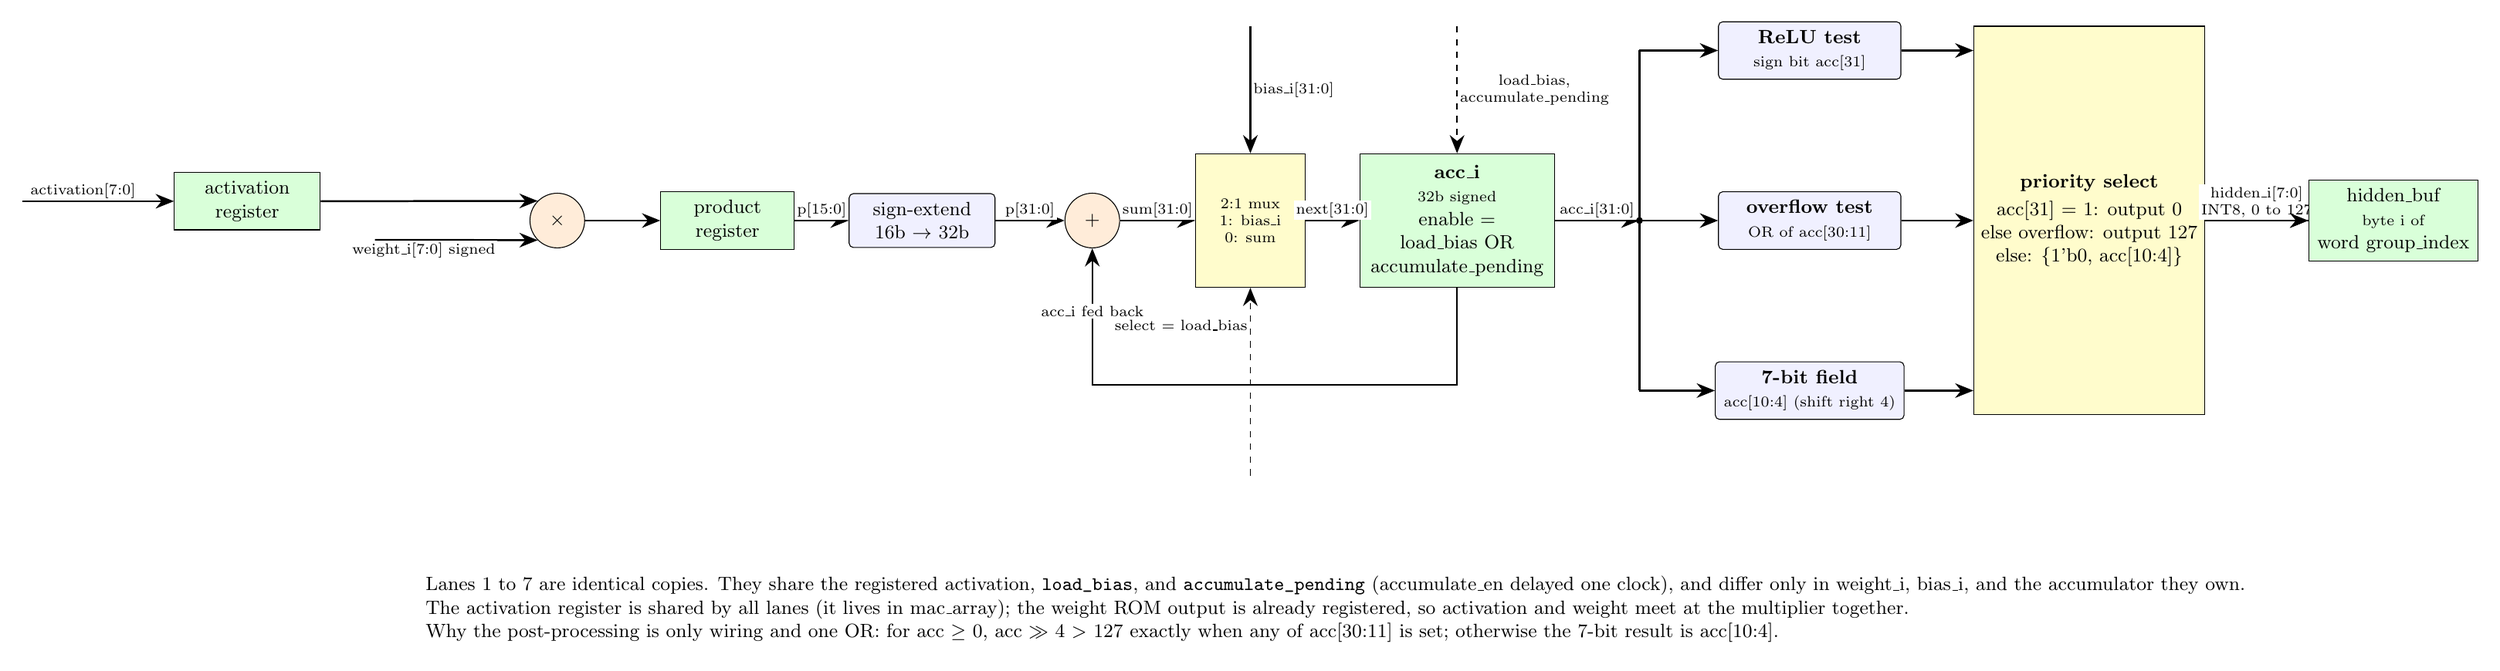
\begin{tikzpicture}
\node[reg,minimum width=2.4cm] (areg) at (-3.9,0.318) {activation\\register};
\node[op] (mul) at (1.2,0) {$\times$};
\node[reg,minimum width=2.2cm] (preg) at (4.0,0) {product\\register};
\node[box,minimum width=2.4cm] (se) at (7.2,0) {sign-extend\\16b $\to$ 32b};
\node[op] (add) at (10.0,0) {$+$};
\node[mux,minimum width=1.8cm,minimum height=2.2cm] (mx) at (12.6,0) {2:1 mux\\1: bias_i\\0: sum};
\node[reg,minimum width=3.2cm,minimum height=2.2cm] (ar) at (16.0,0) {\textbf{acc_i}\\\scriptsize 32b signed\\enable =\\load_bias OR\\accumulate_pending};

\draw[data] (-7.6,0.318) -- node[above,pos=0.4,lab]{activation[7:0]} (areg.west);
\draw[data] (areg.east) -- (mul.north west);
\draw[data] (-1.8,-0.318) -- node[below,pos=0.3,lab]{weight_i[7:0] signed} (mul.south west);
\draw[data] (mul) -- (preg);
\draw[data] (preg) -- node[above,lab]{p[15:0]} (se);
\draw[data] (se) -- node[above,lab]{p[31:0]} (add);
\draw[data] (add) -- node[above,lab]{sum[31:0]} (mx);
\draw[data] (mx) -- node[above,lab]{next[31:0]} (ar);
\draw[data] (12.6,3.2) -- node[right,lab]{bias_i[31:0]} (mx.north);
\draw[ctrl] (12.6,-4.2) -- node[pos=0.8,left,lab]{select = load_bias} (mx.south);
\draw[ctrl] (16.0,3.2) -- node[right,lab]{load_bias,\\accumulate_pending} (ar.north);
\draw[data] (ar.south) -- ++(0,-1.6) -| node[pos=0.8,below,lab]{acc_i fed back} (add.south);

\draw[data] (ar.east) -- node[above,lab]{acc_i[31:0]} (19.0,0);
\draw[very thick] (19.0,2.8) -- (19.0,-2.8);
\fill (19.0,0) circle (1.6pt);

\node[box,minimum width=3.0cm] (s1) at (21.8,2.8)  {\textbf{ReLU test}\\\scriptsize sign bit acc[31]};
\node[box,minimum width=3.0cm] (s2) at (21.8,0)    {\textbf{overflow test}\\\scriptsize OR of acc[30:11]};
\node[box,minimum width=3.0cm] (s3) at (21.8,-2.8) {\textbf{7-bit field}\\\scriptsize acc[10:4] (shift right 4)};
\draw[data] (19.0,2.8) -- (s1.west);
\draw[data] (19.0,0)   -- (s2.west);
\draw[data] (19.0,-2.8) -- (s3.west);

\node[mux,minimum width=3.8cm,minimum height=6.4cm,font=\small] (pm) at (26.4,0) {\textbf{priority select}\\[2pt]acc[31] = 1: output 0\\else overflow: output 127\\else: \{1'b0, acc[10:4]\}};
\draw[data] (s1.east) -- (pm.west |- s1.east);
\draw[data] (s2.east) -- (pm.west |- s2.east);
\draw[data] (s3.east) -- (pm.west |- s3.east);
\draw[data] (pm.east) -- node[above,lab]{hidden_i[7:0]\\INT8, 0 to 127} (30.0,0);
\node[reg,minimum width=2.6cm] (hbo) at (31.4,0) {hidden_buf\\\scriptsize byte i of\\word group_index};
\draw[data] (30.0,0) -- (hbo.west);

\node[align=left,font=\small] at (14,-6.4) {Lanes 1 to 7 are identical copies. They share the registered activation, \texttt{load_bias}, and \texttt{accumulate_pending} (accumulate_en delayed one clock), and differ only in weight_i, bias_i, and the accumulator they own.\\
The activation register is shared by all lanes (it lives in mac_array); the weight ROM output is already registered, so activation and weight meet at the multiplier together.\\
Why the post-processing is only wiring and one OR: for acc $\geq$ 0, acc $\gg$ 4 $>$ 127 exactly when any of acc[30:11] is set; otherwise the 7-bit result is acc[10:4].};
\end{tikzpicture}}
\end{center}

\clearpage
%==========================================================================
{\Large\bfseries 4. Low level: argmax}

\medskip
\begin{center}
\resizebox{0.85\textwidth}{!}{%
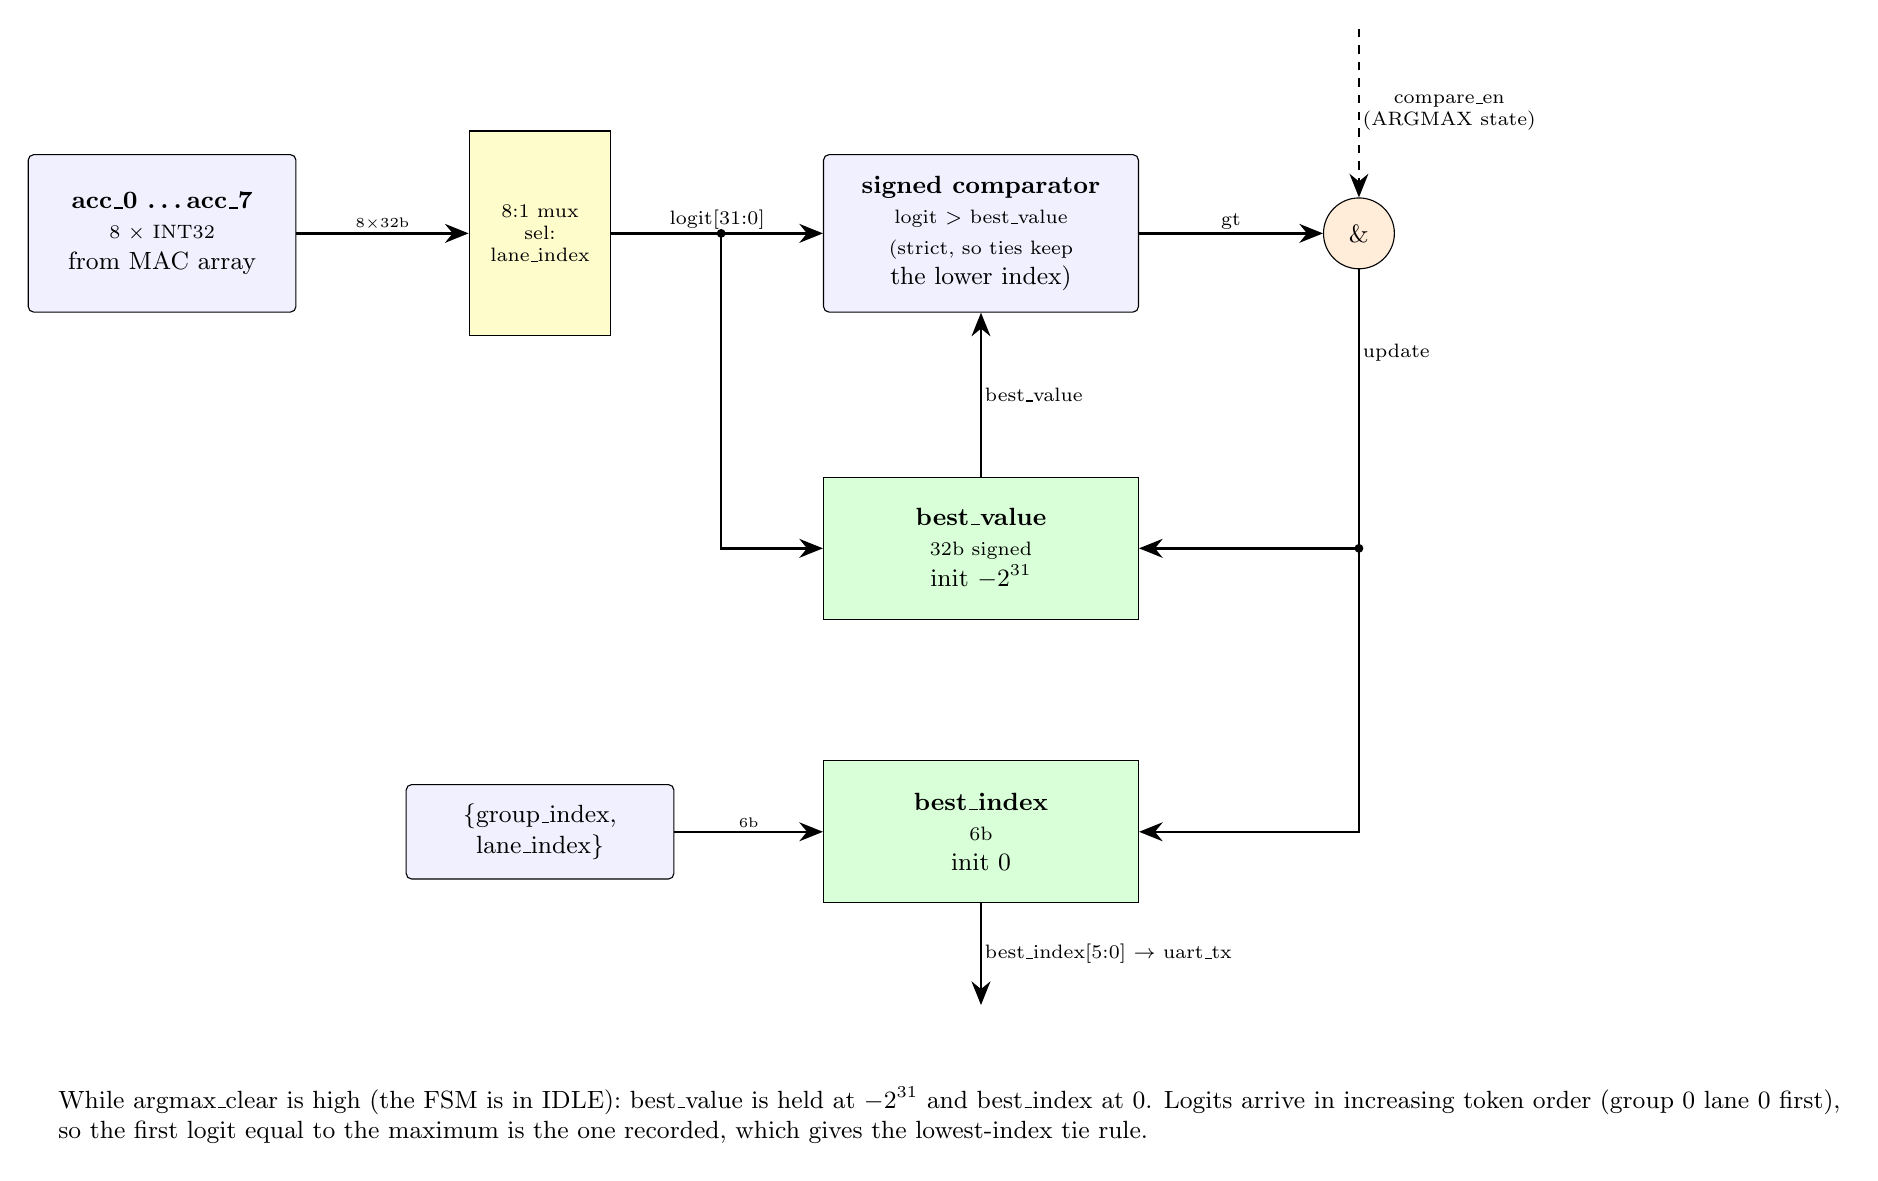
\begin{tikzpicture}
\node[box,minimum width=3.4cm,minimum height=2.0cm] (acc) at (0,0) {\textbf{acc_0 \dots acc_7}\\\scriptsize 8 $\times$ INT32\\from MAC array};
\node[mux,minimum width=1.8cm,minimum height=2.6cm] (m8) at (4.8,0) {8:1 mux\\sel:\\lane_index};
\node[box,minimum width=4.0cm,minimum height=2.0cm] (cmp) at (10.4,0) {\textbf{signed comparator}\\{\scriptsize logit $>$ best_value}\\\scriptsize (strict, so ties keep\\the lower index)};
\node[op] (and) at (15.2,0) {\&};

\draw[data] (acc) -- node[above,lbs]{8$\times$32b} (m8);
\draw[data] (m8) -- node[above,lab]{logit[31:0]} (cmp);
\draw[data] (cmp) -- node[above,lab]{gt} (and);
\draw[ctrl] (15.2,2.6) -- node[right,lab]{compare_en\\(ARGMAX state)} (and.north);

\node[reg,minimum width=4.0cm,minimum height=1.8cm] (bv) at (10.4,-4.0) {\textbf{best_value}\\\scriptsize 32b signed\\init $-2^{31}$};
\node[reg,minimum width=4.0cm,minimum height=1.8cm] (bi) at (10.4,-7.6) {\textbf{best_index}\\\scriptsize 6b\\init 0};
\node[box,minimum width=3.4cm,minimum height=1.2cm] (cat) at (4.8,-7.6) {\{group_index,\\lane_index\}};

\draw[data] (bv.north) -- node[right,lab]{best_value} (cmp.south);
\draw[data] (7.1,0) -- (7.1,-4.0) -- (bv.west);
\fill (7.1,0) circle (1.6pt);
\draw[data] (cat) -- node[above,lbs]{6b} (bi);
\draw[data] (and.south) -- node[pos=0.3,right,lab]{update} (15.2,-4.0) -- (bv.east);
\draw[data] (15.2,-4.0) -- (15.2,-7.6) -- (bi.east);
\fill (15.2,-4.0) circle (1.6pt);
\draw[data] (bi.south) -- node[right,lab]{best_index[5:0] $\to$ uart_tx} (10.4,-9.8);

\node[align=left,font=\small] at (10,-11.2) {While argmax_clear is high (the FSM is in IDLE): best_value is held at $-2^{31}$ and best_index at 0. Logits arrive in increasing token order (group 0 lane 0 first),\\
so the first logit equal to the maximum is the one recorded, which gives the lowest-index tie rule.};
\end{tikzpicture}}
\end{center}

\clearpage
%==========================================================================
{\Large\bfseries 5. Low level: control (state register, flags, counters, output decode)}

\medskip
\begin{center}
\resizebox{\textwidth}{!}{%
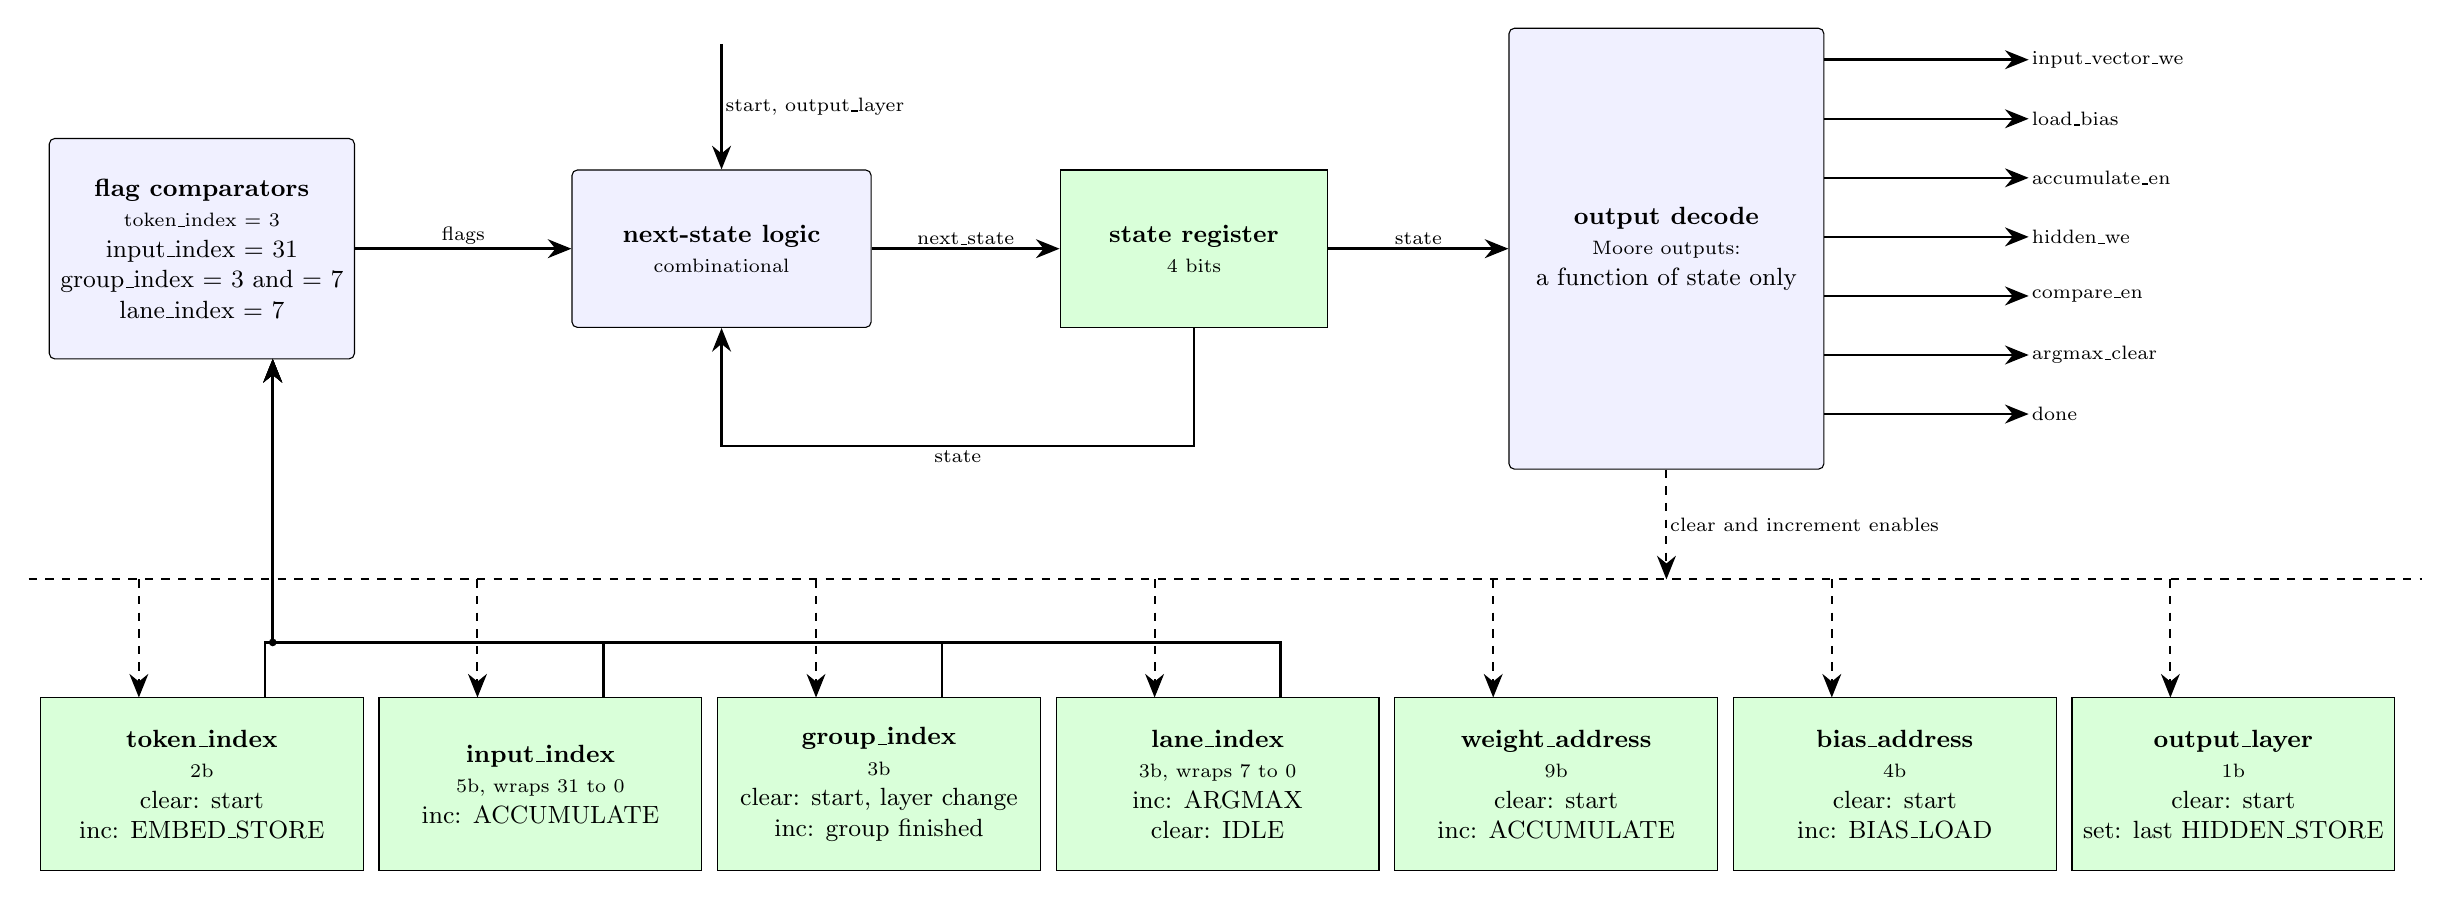
\begin{tikzpicture}
\node[box,minimum width=3.8cm,minimum height=2.8cm] (cmp) at (0,4) {\textbf{flag comparators}\\\scriptsize token_index = 3\\input_index = 31\\group_index = 3 and = 7\\lane_index = 7};
\node[box,minimum width=3.8cm,minimum height=2.0cm] (ns) at (6.6,4) {\textbf{next-state logic}\\{\scriptsize combinational}};
\node[reg,minimum width=3.4cm,minimum height=2.0cm] (sr) at (12.6,4) {\textbf{state register}\\{\scriptsize 4 bits}};
\node[box,minimum width=4.0cm,minimum height=5.6cm] (od) at (18.6,4) {\textbf{output decode}\\\scriptsize Moore outputs:\\a function of state only};

\draw[data] (cmp) -- node[above,lab]{flags} (ns);
\draw[data] (ns) -- node[above,lab]{next_state} (sr);
\draw[data] (sr) -- node[above,lab]{state} (od);
\draw[data] (sr.south) -- ++(0,-1.5) -| node[pos=0.25,below,lab]{state} (ns.south);
\draw[data] (6.6,6.6) -- node[right,lab]{start, output_layer} (ns.north);

\foreach \yy/\nm in {6.4/input_vector_we,5.65/load_bias,4.9/accumulate_en,4.15/hidden_we,3.4/compare_en,2.65/argmax_clear,1.9/done}{
  \draw[data] (20.6,\yy) -- (23.2,\yy);
  \node[lab,anchor=west] at (23.2,\yy) {\nm};
}

\foreach \x/\t in {0/{\textbf{token_index}\\\scriptsize 2b\\clear: start\\inc: EMBED_STORE},
                   4.3/{\textbf{input_index}\\\scriptsize 5b, wraps 31 to 0\\inc: ACCUMULATE},
                   8.6/{\textbf{group_index}\\\scriptsize 3b\\clear: start, layer change\\inc: group finished},
                   12.9/{\textbf{lane_index}\\\scriptsize 3b, wraps 7 to 0\\inc: ARGMAX\\clear: IDLE},
                   17.2/{\textbf{weight_address}\\\scriptsize 9b\\clear: start\\inc: ACCUMULATE},
                   21.5/{\textbf{bias_address}\\\scriptsize 4b\\clear: start\\inc: BIAS_LOAD},
                   25.8/{\textbf{output_layer}\\\scriptsize 1b\\clear: start\\set: last HIDDEN_STORE}}{
  \node[reg,minimum width=4.1cm,minimum height=2.2cm] (c\x) at (\x,-2.8) {\t};
}
\draw[ctrl,-] (-2.2,-0.2) -- (28.2,-0.2);
\draw[ctrl] (od.south) -- node[right,lab]{clear and increment enables} (18.6,-0.2);
\foreach \x in {0,4.3,8.6,12.9,17.2,21.5,25.8}{
  \draw[ctrl] (\x-0.8,-0.2) -- (\x-0.8,-1.7);
}
\foreach \x in {0,4.3,8.6,12.9}{
  \draw[data] (\x+0.8,-1.7) -- (\x+0.8,-1.0) -- (0.9,-1.0) -- (0.9,2.6);
}
\fill (0.9,-1.0) circle (1.4pt);
\end{tikzpicture}}
\end{center}

\vspace{-2pt}
\small
\begin{tabular}{@{}>{\ttfamily}l p{14cm}@{}}
\toprule
\textbf{Control output} & \textbf{Asserted in state, and what it enables} \\
\midrule
input_vector_we & EMBED_STORE: writes embed_data into input_vector word token_index \\
load_bias & BIAS_LOAD: every accumulator loads its bias \\
accumulate_en & ACCUMULATE: every accumulator adds activation $\cdot$ weight$_i$ \\
hidden_we & HIDDEN_STORE: writes the 8 post-processed bytes into hidden_buf word group_index \\
compare_en & ARGMAX: lets the comparator update best_value and best_index \\
argmax_clear & IDLE: holds best_value at $-2^{31}$ and best_index at 0 \\
done & DONE: starts uart_tx with best_index (it must be latched here, since IDLE clears it) \\
\bottomrule
\end{tabular}

\end{document}
